\documentclass[12pt,reqno,sumlimits]{amsart}

 \usepackage{amssymb,amscd,amsmath,epsfig}


%% Two packages to facilitate editing - Fabián.
%\usepackage[mathlines]{lineno}
%\usepackage[dvips,dvipsnames]{xcolor}
\usepackage{graphicx,type1cm,eso-pic}
%%%%%%%%%%%%%%%%%%%%%%%%%%%   

%\usepackage[usenames]{color}
%\def\steve{\textcolor{blue}}
%\def\stevered{\textcolor{red}}


\input Heading.tex

  \newcommand{\BbR}{{\mathbb R}}
\newcommand{\BbP}{{\mathbb P}}
 \newcommand{\BbC}{{\mathbb C}}
 \newcommand{\BbZ}{{\mathbb Z}}
 \newcommand{\pdo}{\Psi{\rm DO}}
 \newcommand{\pdos}{\pdo^*}
 \newcommand{\calg}{{\mathfrak g}}
 \newcommand{\gl}{{\mathfrak gl}}
 \newcommand{\e}{\varepsilon}
 \newcommand{\dvol}{{\rm dvol}}
 \newcommand{\oo}{{\rm o}}
 \newcommand{\OO}{{\rm O}}
 \newcommand{\nlc}{\nabla^{\rm LC}}
 
 \newcommand{\diffm}{{\rm Diff}(M) }
 \newcommand{\diffo}{{\rm Diff}({\overline{M}_p})}
 \newcommand{\diff}{{\rm Diff} }
 \newcommand{\maps}{{\rm Maps} }
 \newcommand{\kk}{2k-1 }
 
 \newcommand{\resw}{{\rm res}^{ W}}
 
 \newcommand{\be}{\overline\eta}
  \newcommand{\bn}{\overline\nabla}
  \newcommand{\bxi}{\overline\xi}
    \newcommand{\bxis}{\overline\xi^*}
\newcommand{\br}{\overline R}
\newcommand{\bmk}{\overline{ M}_p}
\newcommand{\bg}{\overline g}
\newcommand{\bx}{\overline X}
\newcommand{\by}{\overline Y}
\newcommand{\bz}{\overline Z}
\newcommand{\bp}{\overline \Phi}
\newcommand{\bm}{\overline m}
\newcommand{\ocs}{\widetilde{CS}}
\newcommand{\tp}{\tilde p}
\newcommand{\xl}{X^L}
\newcommand{\yl}{Y^L}
\newcommand{\zl}{Z^L}
\newcommand{\la}{\langle}
\newcommand{\ra}{\rangle}
\newcommand{\sgn}{{\rm sgn}}
\newcommand{\dg}{\dot\gamma}
\newcommand{\ints}{\int_{S^1}}

\newcommand{\eb}{\overline e}
\newcommand{\ebo}{\eb_{\sigma(1)}}
\newcommand{\ebt}{\eb_{\sigma(2)}}
\newcommand{\ebth}{\eb_{\sigma(3)}}
\newcommand{\ebf}{\eb_{\sigma(4)}}
\newcommand{\ebfi}{\eb_{\sigma(5)}}

\newcommand{\el}{e^L}
\newcommand{\elt}{e^L_{\sigma(2)}}
\newcommand{\elth}{e^L_{\sigma(3)}}
\newcommand{\elf}{e^L_{\sigma(4)}}
\newcommand{\elfi}{e^L_{\sigma(5)}}

\newcommand{\eet}{e_{\sigma(2)}}
\newcommand{\eeth}{e_{\sigma(3)}}
\newcommand{\eef}{e_{\sigma(4)}}
\newcommand{\eefi}{e_{\sigma(5)}}

\newcommand{\aoa}{A_{1a}}
\newcommand{\aob}{A_{1b}}
\newcommand{\aoc}{A_{1c}}


\newcommand{\ssum}{ \sum_{\sigma(1) = 1}\sgn(\sigma)}
\newcommand{\vol}{{\rm vol}}
\newcommand{\omp}{\overline{M}_p}
\newcommand{\ompc}{\overline{M}_{p,c}}
\newcommand{\mab}{\overline {M}_{(a,b)} }
\newcommand{\mabp}{\overline {M}_{p(a,b)} }

\newcommand{\tid}{\rm Id}

\newcommand{\wgti}{ (1+\Delta)^{-1}}

\newcommand{\chk}{ch^W_{[2k]}}
\newcommand {\PD}{{\rm PD}}
\newcommand{\cp}{\mathbb C\mathbb P}



\begin{document}

\newpage\null\vskip-4em
  \noindent\scriptsize{}
  \scriptsize{
 %%%%%%%%%%%%%%% comment out if undesired and uncomment \textsc{}} line
 % \textsc{AMS Mathematics Subject
%  Classification Numbers: 58J28, 58J40.
%} }
\vskip 0.5 in


\normalsize



\title[Computation for diffeomorphism groups of circle bundles]{Computation for Diffeomorphism groups of circle bundles over integral 
K\"ahler and symplectic manifolds}
\author[S. Egi]{Satoshi Egi}
\address{Rakuten Institute of Technology}
\email{egi@egison.org}
\author[Y. Maeda]{Yoshiaki Maeda}
\address{Tohoku Center for Creativity\\
Tohoku University}
\email{yoshimaeda@m.tohoku.ac.jp}
\author[S. Rosenberg]{Steven Rosenberg}
\address{Department of Mathematics and Statistics\\
  Boston University}
\email{sr@math.bu.edu}







\maketitle
%Comment the next line and un-comment second line to change color of text from red to black
\definecolor{ColorEdit}{named}{red}
%\definecolor{ColorEdit}{named}{black}


%Comment next line to eliminate line numbers
%\pagewiselinenumbers

\section{\bf Introduction}

This article presents a program for computing Wodzicki-Chern-Simons form of certain K\"ahler manifold with the Egison programming language.

\section{\bf Computation}

\begin{figure}[]
\begin{center}
  \fbox{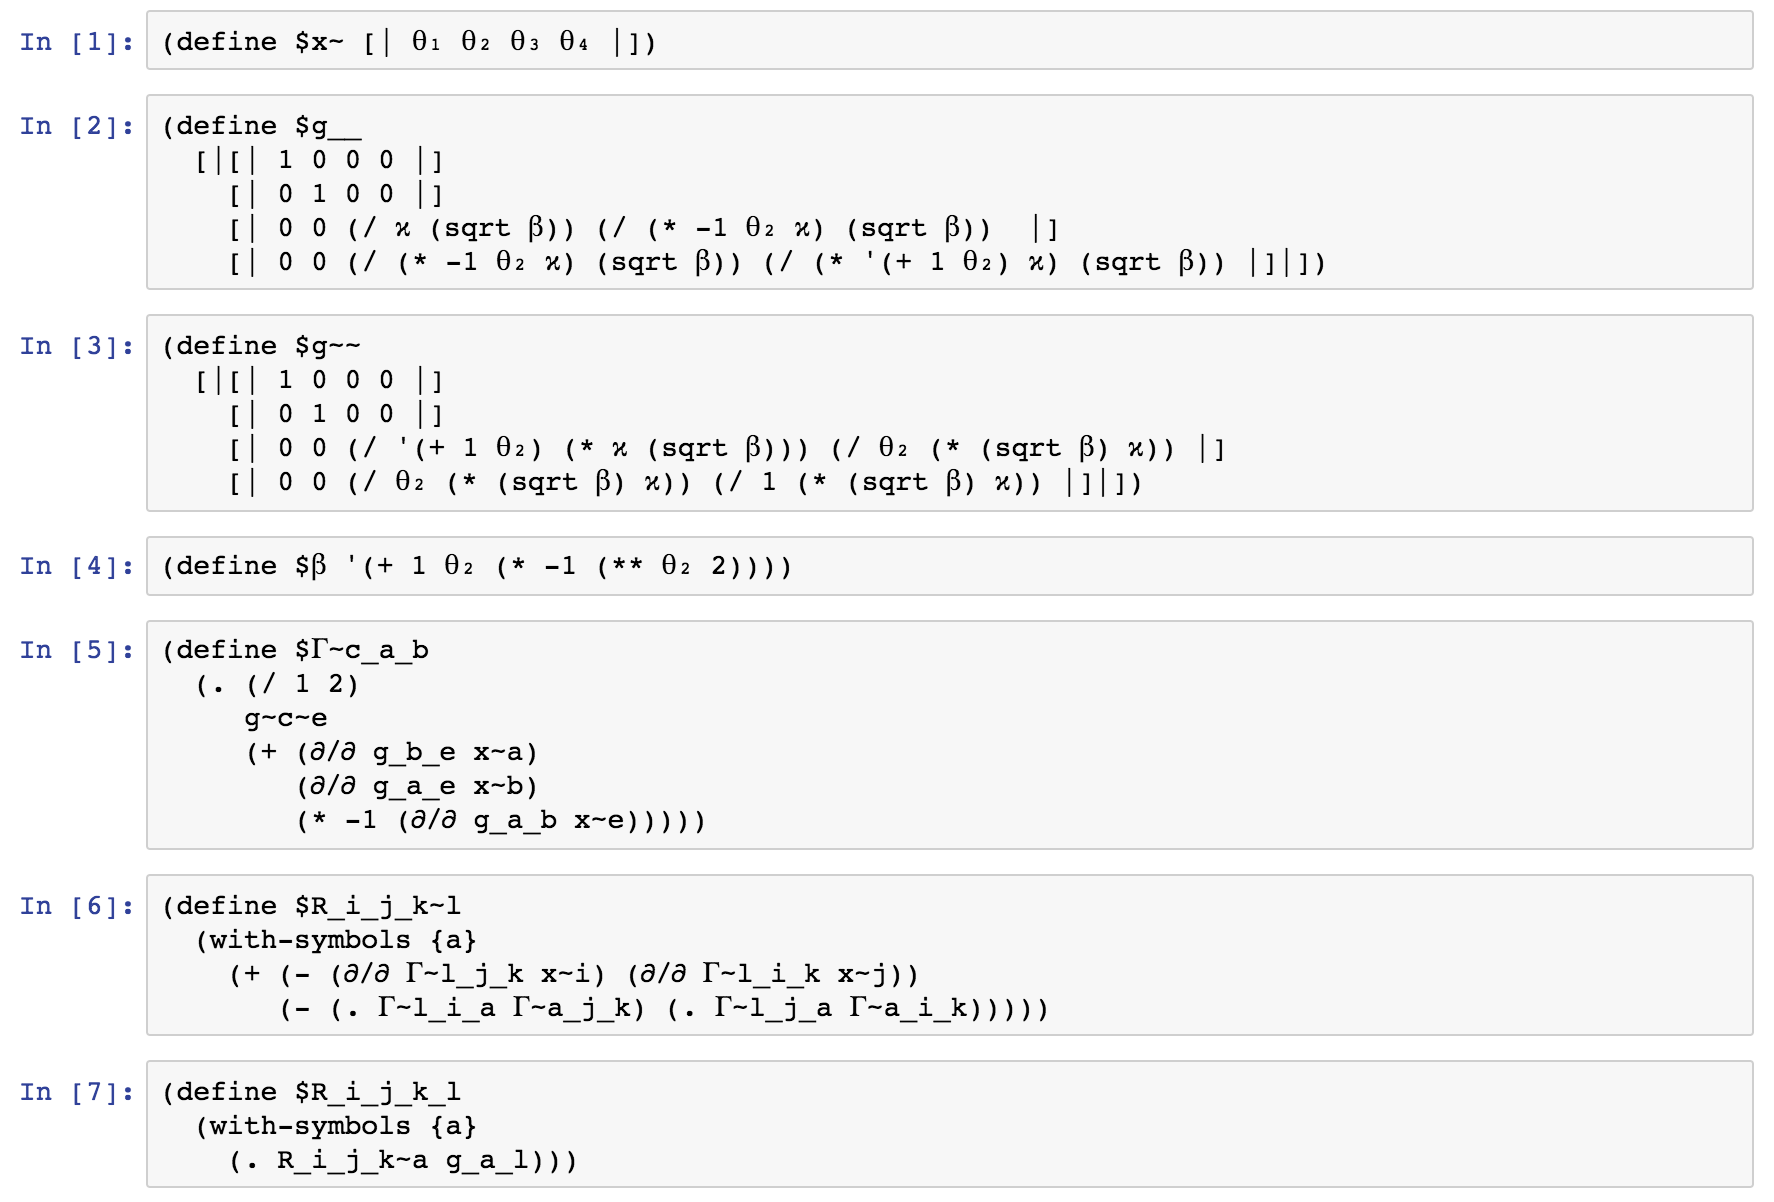
\includegraphics[width=15cm,bb=0 0 887 601]{images/program1-7.png}}
\end{center}  
%\caption{Metrics and Riemann curvature}
\label{fig:program1-7}
\end{figure}

\begin{figure}[]
\begin{center}
  \fbox{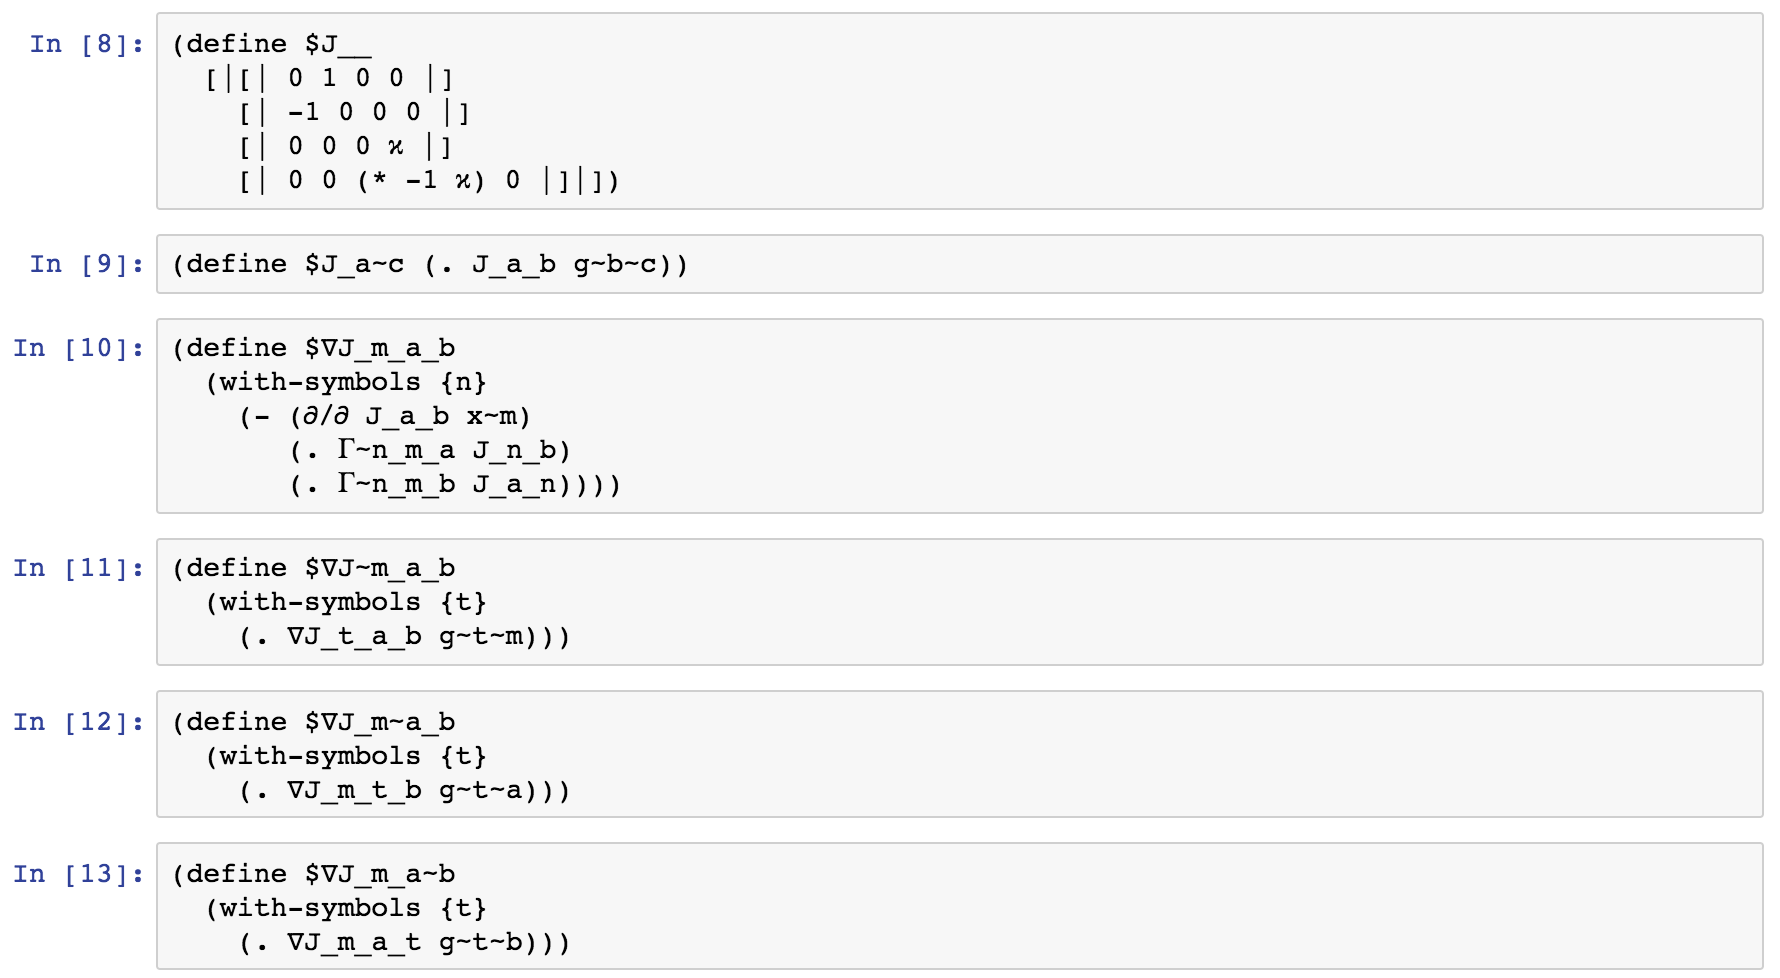
\includegraphics[width=15cm,bb=0 0 890 489]{images/program8-13.png}}
\end{center}  
%\caption{}
\label{fig:program8-13}
\end{figure}

\begin{figure}[]
\begin{center}
  \fbox{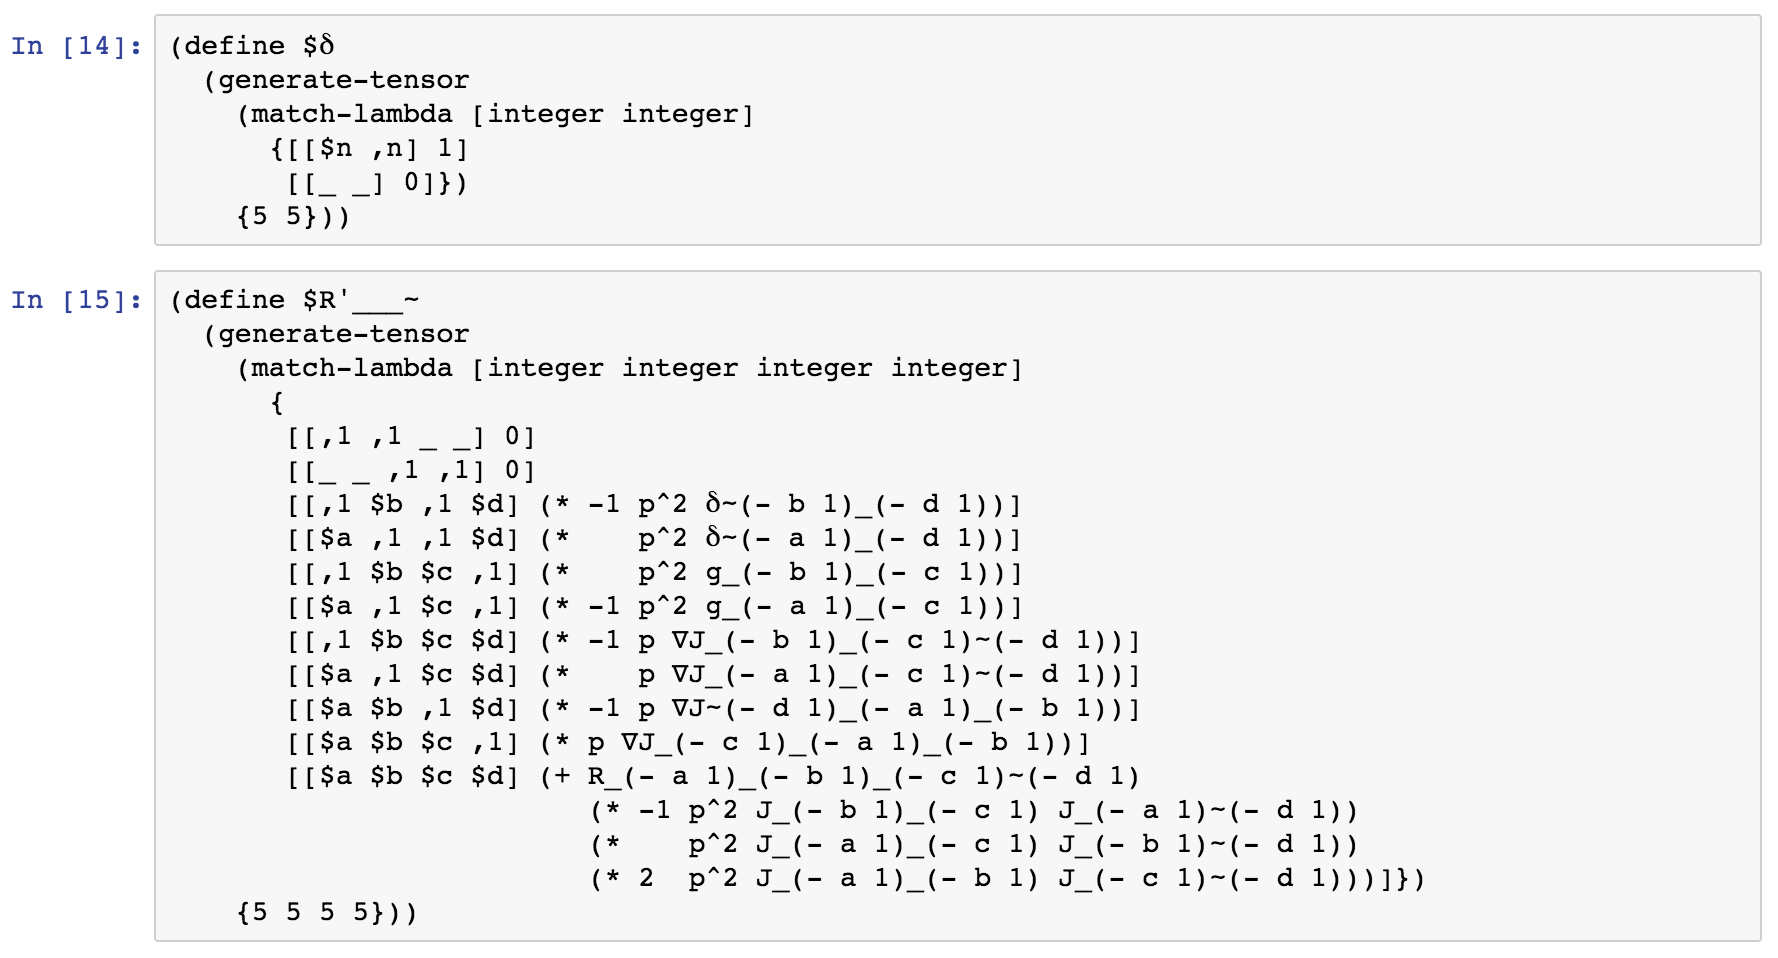
\includegraphics[width=15cm,bb=0 0 889 479]{images/program14-15.png}}
\end{center}  
%\caption{}
\label{fig:program14-15}
\end{figure}

\begin{figure}[]
\begin{center}
  \fbox{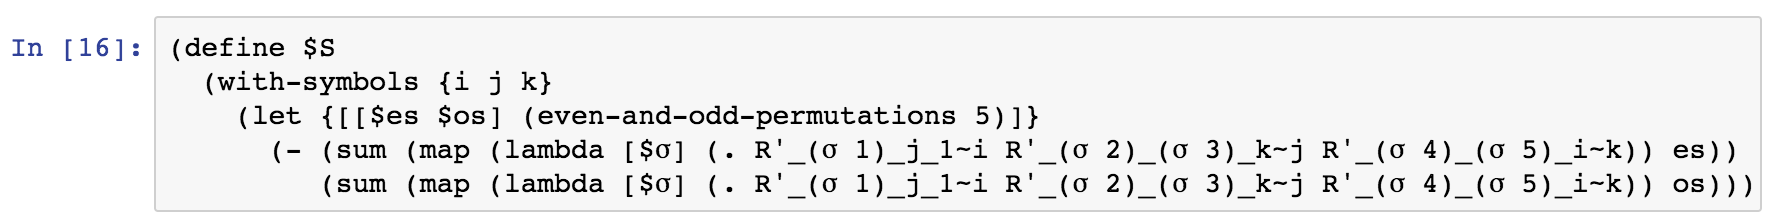
\includegraphics[width=15cm,bb=0 0 887 112]{images/program16.png}}
\end{center}  
%\caption{}
\label{fig:program16}
\end{figure}


{\footnotesize
\begin{verbatim}
\end{verbatim}
}


\end{document}
